\chapter{Making Decisions} 

\section{Introduction} 

At the end of the previous chapter we saw how we could get the user to type something in, and then advance the story. In this chapter, we explore this further. We start with the user simply pressing \emph{Enter} to advance the story, just like turning a page. Then, we look at \textit{variables}, for example \textit{String} variables that can hold text. We use a variable to pick up what the player just typed in -- remember \texttt{command}? Once we have that, we inspect what the player wants to do (e.g. look around, or go south) and drive the story forward accordingly. For that, you learn more about the \texttt{if..then..else} control structure in Python, and basic String comparison \texttt{==}. By the end of the chapter, we will have a game where the player can roam around various rooms in the house, look around, and find all manner of horrific things ... 

\section{The Story So Far} 

So far, the story is that you are in "a dark, spooky house, all alone out in the forest." Scary thing is, you are inside -- and you cannot get out! Whereas, hearing strange noises, getting out is clearly what you want ... 

 \begin{Gmd}[Victory condition] Most games have a \textit{\victorycondition}: What you need to achieve to win the game. Collect all the little shiny boxes, like in \emph{Fez}, or defeat all the monsters, like in \emph{Dark Souls}, or free the princess in \emph{Super Mario}. (Not all games have apparent victory conditions, for example look at an exploration game like \emph{Dear Esther}.) Key is of course that the player has some idea about what the victory condition might be. In our story, the first few lines already make it clear: Escape! Which then turns into the question, how ....  \expend  
  \end{Gmd} 
  
  Having some idea about what you need to achieve is good, but even better is knowing \emph{how} you can achieve it! This is where \gamemechanic{s} and \event{s} come into play (literally).   
      
  \begin{Gmd}[Game mechanics and events] A \textit{\gamemechanic} defines how the game works. It is a rule we implement in code, determining what a player can do. If the player does "this," then "that" is going to happen. For example, many games use the \emph{A} button on the (Xbox) controller to make your character jump. That is a mechanic. Or, in text adventures, you type in a command -- that is another mechanic. When you are playing a game, you use these mechanics to make things, \textit{\event{s}}, happen. Things may go one way or the other, depending on what you decide to do. Take again \emph{Dark Souls} -- as the monster attacks you, do you press \emph{L1} to raise your shield and block the attack, or do you use your left stick and \emph{O} to roll to the side? Different mechanics, allowing you to take different actions, resulting in different ways in which the game might play out ...   \expend
  \end{Gmd}
  
Let's use that to work out our story a little bit more. The \victorycondition\ is to get out of the house but the only door outside is locked. Let's assume that that means the player needs to find a key. As the game wouldn't be particularly exciting if the key would be laying there right in front of the player's nose, we need some \gamemechanic{s} for the user to go around the house, and look for objects. And that should, of course, lead to some "interesting" events ...  

\begin{figure}[h]
\centerline{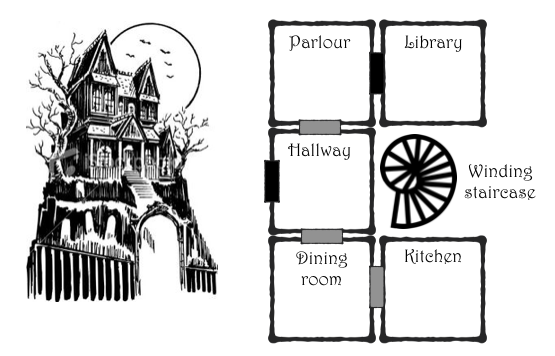
\includegraphics[scale=.70]{images/p1ch2-hauntedhousemap.png}}
\caption{The Haunted House In The Forest}\label{fig:hauntedhousemap}
\end{figure}

\figref{fig:hauntedhousemap} shows the map of the house. The black and grey triangles indicate doors. Grey means these doors are open, black means that door is closed -- the player needs to find the right keys to open it. The player can find the key to the \emph{Library} in the \emph{Parlour}. The key to the door outside is in a handbag in the \emph{Kitchen}. 

Now, this would not be a scary story if there would not be any monsters around ... So let's place a Ghoul in the kitchen, to guard the Key To Outside. This is going to be our \emph{Boss Fight}! 

We should not allow the user to simply waltz into the kitchen, completely ignore the Ghoul, and just grab the key. No -- if the player does that, "You Died!" Instead the player needs to find a weapon to defeat the Ghoul. The Library is a good place for that. We can put a sword above the mantelpiece. For good measure we also put a Ghost in the Library. The Ghost floats in front of the sword. 

Those are our key objects: the key to get into the Library (found in the Parlour), the sword to kill the Ghoul (found in the Library), and the key to get out of the house . The player can find that final key in a handbag in the Kitchen. To spice things up, we can let the Ghoul carry the handbag around its neck.  

We now have our locations, our objects, a monster -- what we need now still is define what the player can do. 

We have objects, so a player should be able to \textbf{take} an object -- "take sword" or "pick up key." 

We are not going to place these objects in plain sight, as that would be too easy. The player should \textbf{search} -- "search room" or "look in handbag." 

Naturally, the player needs to be able to get around the house. We can do that "old school"-style using \textbf{go} with a compass direction -- "go north", "go south." From the Hallway you can go North to the Parlour, or South to the Dining Room, etcetera. 

Finally, as we have monsters, the player needs to be able to \textbf{attack} a monster -- or \textbf{retreat} if the monster is too scary! 

Okay, there we go. All we need now is the story ... and the code. 

\section{Getting The Story Going} 

Let us have a look again at the code we have so far. 

\begin{lstlisting}
print("You are in a dark, spooky house, all alone out in the forest.")
print("There is only one door to the outside, and it is locked.")
print("You hear strange, creaky sounds.")
command = input("> ")
print("Boo!")
\end{lstlisting}

As our story is going to continue well beyond the cheap jump scare in line 5, we can delete the "Boo!" Instead, we should take stock of the situation. What do we know? Well, we know that the player does \emph{not} have the main key, nor the key to the library, nor the sword -- nor the handbag for that matter. All of that is key to achieving the victory condition: 

\begin{enumerate}
\item Search the Parlour to find the key to the Library
\item In the library, attack the Ghost, then take the sword
\item In the kitchen, use the sword to attack the Ghoul
\item After the Ghoul has been defeated, take the handbag
\item Search the handbag, find the main key
\end{enumerate} 

Once the player has the main key, he should go to the Hallway, and escape the haunted house. Game over, "You Win!"

This means we need to track what the player already has. We can use variables for that. A variable is essentially a "container" you can put a value in (assign a value to). For example, look at line 4 again: 

\begin{verbatim}
command = input("> ")
\end{verbatim}      

We introduce here a variable \texttt{command}, to which we assign a value we get from the function \texttt{input} -- i.e. command stores what the user has just typed in. In Python, there are various types of variables. The \texttt{command} variable is a variable of type \textit{\strvar}. A \strvar\ stores text. If the user types in \textit{go south} and presses enter, then the \emph{value} of \texttt{command} becomes 'go south'. 

\begin{Exe} 
Try this out in \texttt{idle}. Type line 4 in \texttt{idle}, and then type in a command. After you have pressed enter, type in \texttt{command} (the variable name), and press enter again. \texttt{idle} shows the value assigned to that variable.  \expend
\end{Exe}

There are also various other types of variables. Two types you will frequently encounter are \textit{\integer} variables, and \textit{\boolean} variables. An \integer\ variable stores (whole) numbers. 

 \begin{Exe} 
Try this out in \texttt{idle}. Type in \texttt{score = 0}. You have zero points! To check that, type in \texttt{score} (and press enter), and you will see -- 0. If you want a higher score than that, simply add that to the variable, like so: \texttt{score = score + 100}. This means, "take the current score, add 100, and store the resulting number again in score." Now add another 10 points, and check what value is assigned to \texttt{score}. \expend
\end{Exe}

\begin{Exp}[Integer addition short cut] 
If all you want to do is add a number to the current value of an \integer\ variable, and assign the result again to that variable, (like we did above), then Python has a shortcut for that. Instead of \texttt{score = score + 100} you can also use the short-cut \texttt{score += 100}. \expend
\end{Exp} 
 
A \boolean\ variable is a variable that is either \texttt{True} or \texttt{False}. 

\begin{Exp}[Flags] 
Sometimes we call such \boolean\ variables "\flag{s}"  A flag variable is a variable you define to have one value until some condition is true, in which case you change the variable's value. For example, \texttt{hasSword = False} until the player has taken the sword in the Library -- then it becomes \texttt{True}.  It is a variable you can use to control the flow of a function or statement, allowing you to check for certain conditions. So, only once it is the case that \texttt{hasSword = True}, the player can attack the Ghoul and stand a chance to survive that encounter. \expend
\end{Exp} 





 






 

 

      


 



  